%-------------------------------------------------------------------------------------------
	\section{Introduction}
%-------------------------------------------------------------------------------------------

\begin{figure}[htb]
\centering
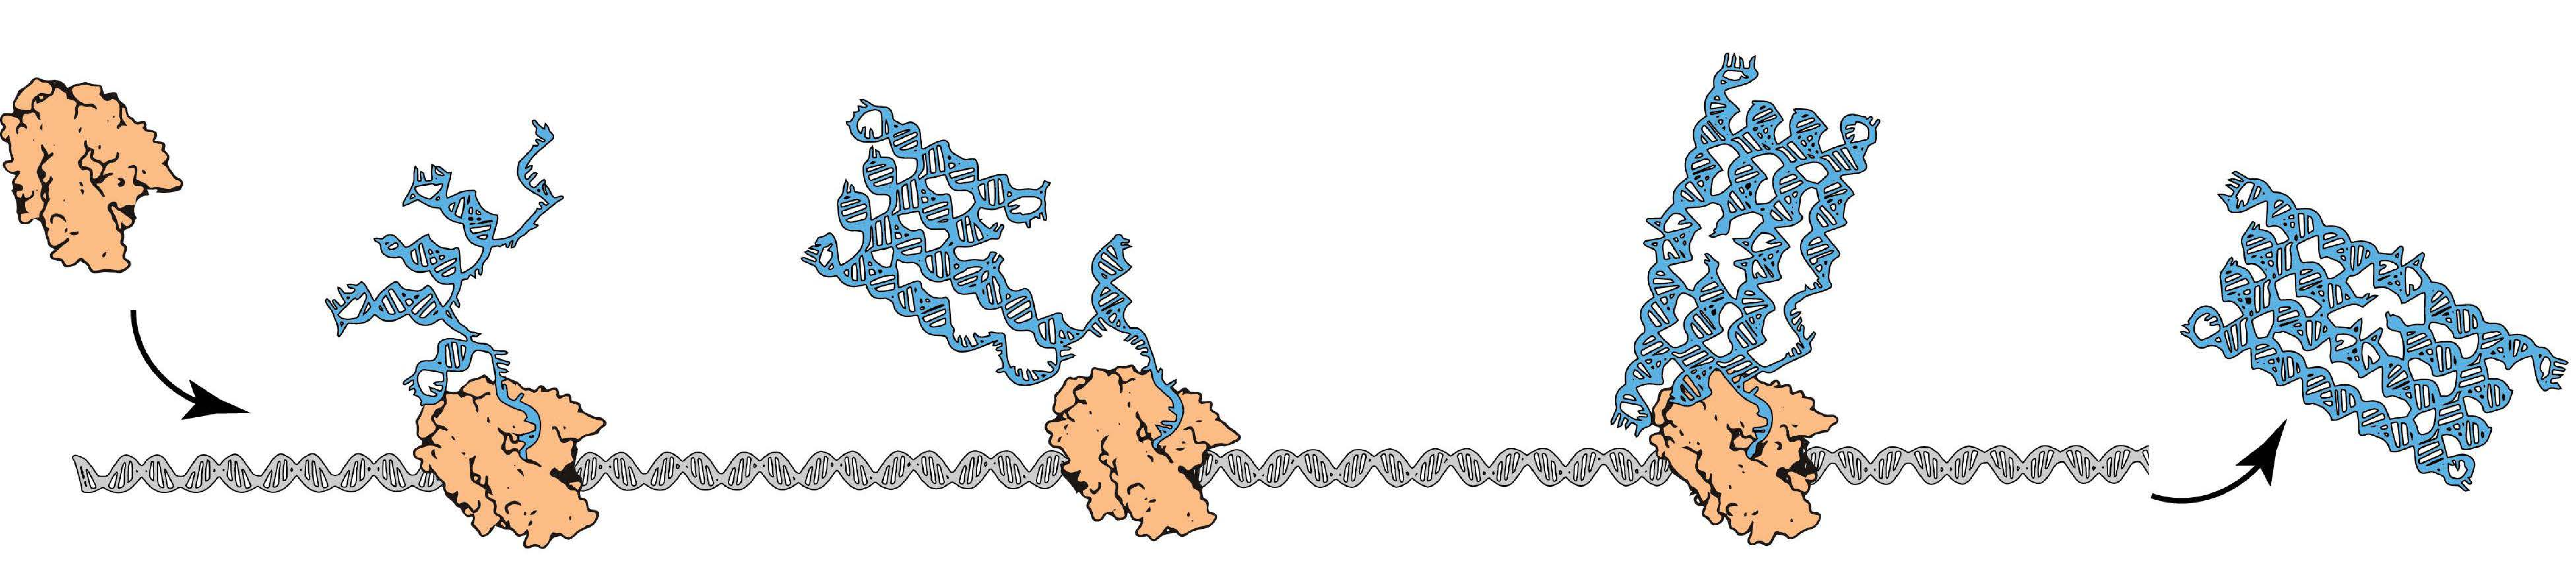
\includegraphics[width=\linewidth]{pic/rna_origami.pdf}
\caption{RNA cotranscriptional folding. 
An RNA polymerase enzyme attaches to a template DNA sequence (gray spiral), scans it through, and synthesizes its RNA copy. 
The RNA sequence begins to fold upon itself immediately as it emerges from the RNA polymerase. 
}
\label{fig:rna_origami}
\end{figure}

An RNA sequence, over nucleotides of four kinds {\tt A}, {\tt C}, {\tt G}, {\tt U}, is synthesized (\textit{transcribed}) from its template DNA sequence over {\tt A}, {\tt C}, {\tt G}, {\tt T} nucleotide by nucleotide by an RNA polymerase (RNAP) enzyme according to the one-to-one mapping ${\tt A} \to {\tt U}$, ${\tt C} \to {\tt G}$, ${\tt G} \to {\tt C}$, and ${\tt T} \to {\tt A}$ (for details, see, e.g., \cite{AJLMRRW2014}). 
The yield, called \textit{transcript}, starts folding immediately after it emerges from RNAP. 
This is the \textit{cotranscriptional folding}. 
Geary, Rothemund, and Andersen have recently demonstrated the capability of cotranscriptional folding to manufacture an RNA molecule of an intended shape at nano-scale \cite{GearyRothemundAndersen2014}. 
They actually proposed an architecture of a DNA sequence whose transcript folds cotranscriptionally into an RNA rectangular tile highly likely \textit{in vitro} (see Figure~\ref{fig:rna_origami}). 

Using a novel computational model of cotranscriptional folding called the \textit{oritatami system} \cite{GeMeScSe2016}, we shall initiate the theoretical study on algorithmic self-assembly of shapes by cotranscriptional folding. 
Algorithms and computation are fundamental to molecular self-assembly as illustrated in an enormous success of their use in DNA tile self-assembly (see, e.g., \cite{Doty2012,Patitz2016,WinfreePhD} and references therein). 
%The concepts of computation and algorithms are yet to be as much utilized in the self-assembly of shapes by cotranscriptional folding as in the DNA tile self-assembly, where for example 
A fractal pattern called Sierpinski triangle was algorithmically self-assembled from coalescence of DNA tiles that compute XOR \cite{RothemundPapadakisWinfree2004}. 
Cotranscriptional folding exhibits highly sophisticated computational and algorithmic behaviors. 
Fluoride riboswitches in the \textit{Bacillus cereus} bacteria cotranscriptionally fold a terminator stem that suppresses gene expression or not, depending on ligand concentration \cite{WaStYuLiLu2016}. 
Cotranscriptional folding is in fact proved Turing-universal by the oritatami system \cite{GeMeScSe2015}. 
The Turing-machine simulator is gigantic and intricate but oritatami systems have implemented basic computational devices such as binary counter \cite{GeMeScSe2016} as a module comparable in size to the gene expression regulator. 
The binary counter module consists of half-adder components, which fold into one of possible four conformations depending on a 1-bit input and a 1-bit carry/non-carry encoded in their surroundings somehow. 
It can be diverted as a copier for binary sequences by being fed with the non-carry. 
They shall be reused in this paper. 

\begin{figure}[htb]
\centering
\begin{minipage}{0.4\linewidth}
\centering
\scalebox{0.8}{\begin{tikzpicture}[>=latex, node distance=2cm, initial text=, bend angle=15]
	\tikzstyle{every initial by arrow} = [->, double];

	\node [state, initial] (q_0)                        {$q_0/R$};
	\node [state]                     (q_1) [right of = q_0]  {$q_1/R$};
	\node [state]                     (q_2) [below right of = q_1] {$q_2/L$};
	\node [state]                     (q_3) [above right of = q_1] {$q_3/R$};

	\path [->] (q_0) edge [right] node [above]              {$0$}                 (q_1)
         		         edge [loop above] node [above]             {$1$}               ()
         			   (q_1) edge [bend left] node [above]             {$0$}                 (q_3)
         		         edge [bend right] node [below]             {$1$}              (q_2)
         			   (q_2)  edge [loop above] node [above]             {$0,1$}               ()
         			   (q_3)  edge [loop above] node [above]             {$0,1$}               ();
\end{tikzpicture}}
\end{minipage}
\begin{minipage}{0.05\linewidth}
\ \\
\end{minipage}
\begin{minipage}{0.5\linewidth}
\centering
\scalebox{0.035}{\begin{tikzpicture}
  \draw[blue!50!black,rotate=270,l-system={rule set={X->X-YF,Y->FX+Y},
  step=100pt,angle=90,axiom=FX,order=10},-triangle 90] l-system;
\end{tikzpicture}}
\end{minipage}
\caption{
Heighway dragon. 
(Left) A DFAO that reads the binary representation of $i$ from the least significant bit and outputs the direction to turn. 
(Right) The 10th iteration of the Heighway dragon, that is, the first $2^{10}-1$ turns of it. 
}
\label{fig:heighway_dragon}
\end{figure}

Algorithmic cotranscriptional folding of Sierpinski triangle would allow oritatami systems to borrow rich insights from the DNA tile self-assembly. 
On the other hand, in order to cut more directly to the heart of algorithmic self-assembly by cotranscriptional folding, we should study the fabrication of shapes that is traversable in some algorithmic way. 
One such way is to feed a turtle program (see \cite{AbelsondiSessa1981}) with a binary \textit{automatic sequence} as commands (drawing a line segment, rotation, etc.), whose $i$-th bit (starting from 0) can be obtained by giving a binary representation of $i$ from the least significant bit to one deterministic finite automaton with output (DFAO) \cite{AlloucheShallit2003}.
%which can be generated by a deterministic finite automaton with output (DFAO) \cite{AlloucheShallit2003}. 
Shapes thus describable include the Heighway dragon \cite{AlloucheShallit2003} and von Koch curve \cite{MaHoldener2005}. 
A DFAO for the Heighway dragon is shown in Figure~\ref{fig:heighway_dragon} (Left). 
It is to read the binary representation of $i \ge 0$ from the least significant bit (LSB) and outputs the $i$-th direction $P[i]$ to turn (R or L) assigned to the state finally reached as follows: 
\[
\begin{array}{cccrrrrc}
i 	&=& 0 &  2 & 6 & 14 & 30 & \cdots \\
P[i] 	&=& {\rm R} & {\rm RL} & {\rm RRLL} & {\rm RRRLLRLL} & {\rm RRRLRRLLLRRLLRLL} & \cdots
\end{array}
\]
where only the values of $i$ at the end of the first five iterations are specified. 
A turtle should interpret an R (resp.~L) as ``move forward by unit distance and turn right (resp. left) 90 degrees.''
The sequence is denoted by $P$ after its appellative \textit{paperfolding sequence} \cite{AlloucheShallit2003}. 

\begin{figure}[htb]
\centering
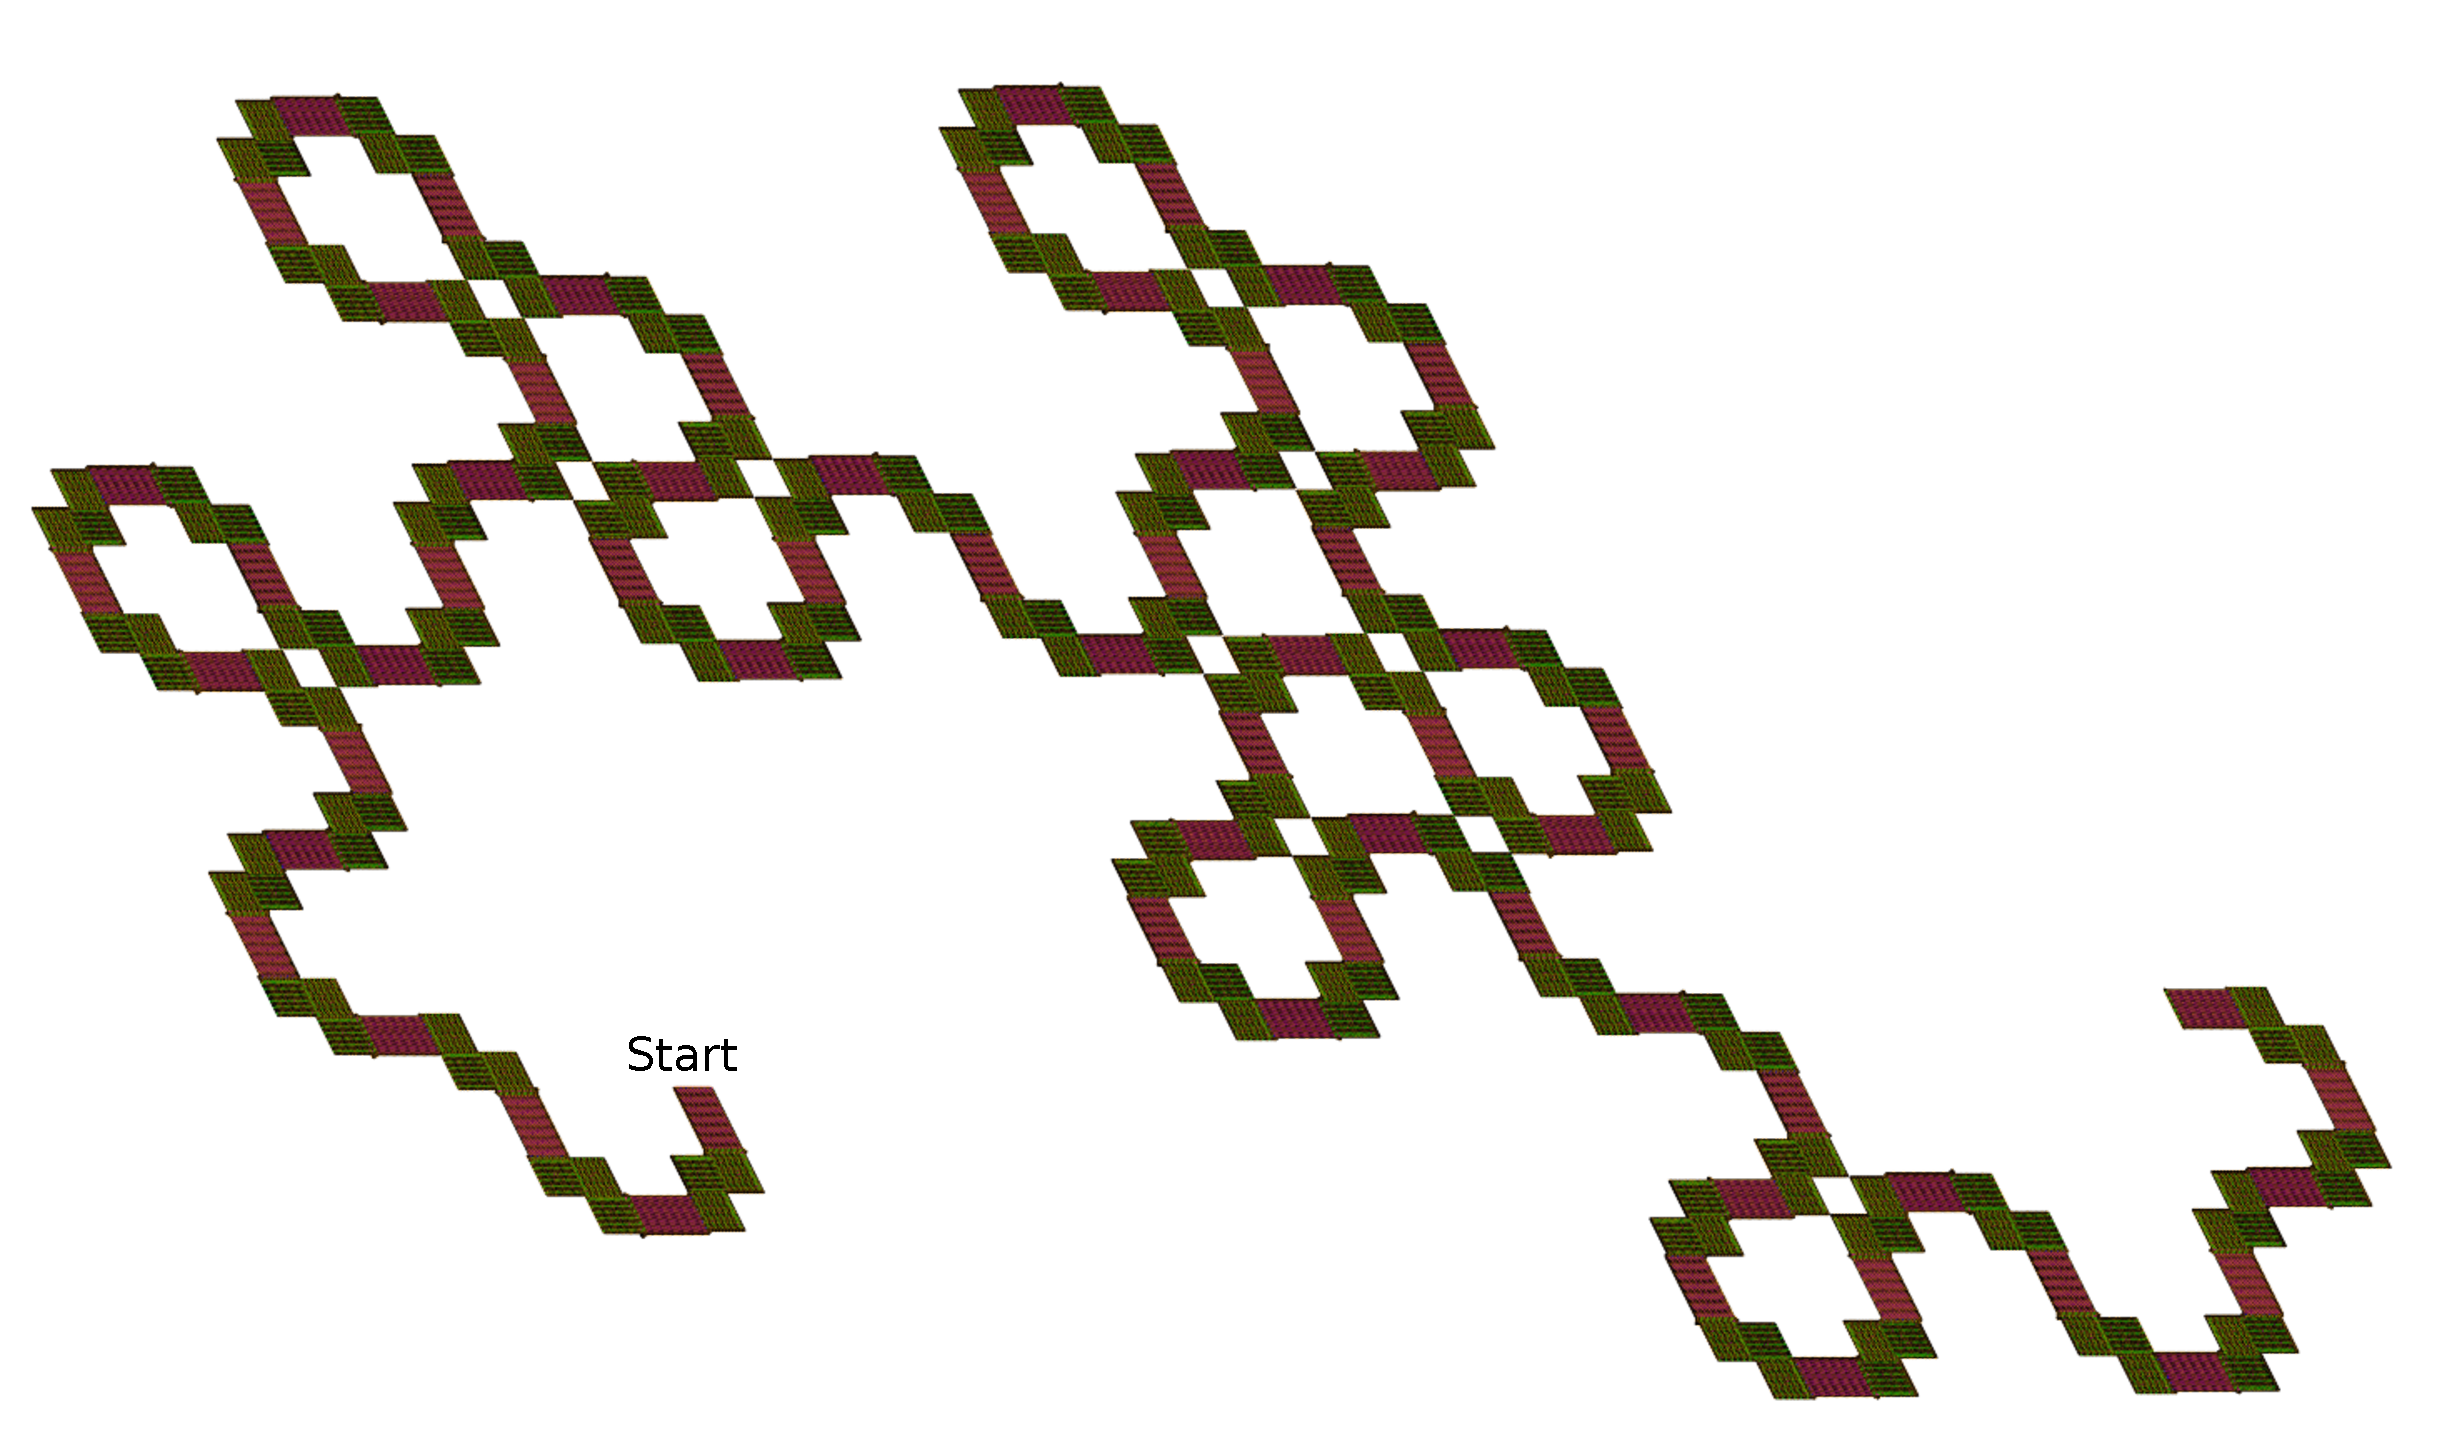
\includegraphics[width=\linewidth]{pic/6bit_heighway.pdf}
\caption{The 6th iteration of the Heighway dragon folded by the proposed oritatami system.}
\label{fig:heighway6_oritatami}
\end{figure}

In this paper, we propose an oritatami system that cotranscriptionally folds into a finite portion of the Heighway dragon. 
Figure~\ref{fig:heighway6_oritatami} shows the 6-th iteration of the Heighway dragon thus folded (the dragon is slanted, but this is because the oritatami system operates on the triangular grid). 
The system consists of four modules: binary counter and copier modules, which are a technical modification of those from \cite{GeMeScSe2016}, DFAO module, and turning module. 
A (red) line segment in Figure~\ref{fig:heighway6_oritatami} consists of a binary counter and copiers, which increment the current count $i$ by 1 and let the count be propagated through. 
At the end of the segment is a DFAO module, which computes $P[i]$, the direction to turn, while forwarding the count $i$ from the last copier to the following turning module. 
A (green) L-shaped block is the turning module. 
A turning module consists of three rhombic components, each of which bifurcates the count $i$ and the direction $P[i]$ leftward as well as rightward and directs the growth of further folding leftward if $P[i] = L$ or rightward if $P[i] = R$. 
We shall implement the DFAO and turning modules and verify them. 

A JavaScript program to execute this oritatami system and websites on which this program is executable are freely available \cite{heighway_web}. 

